\documentclass[11pt,a4paper]{article}
\usepackage[margin=27mm]{geometry}
\usepackage[T1]{fontenc}
\usepackage{mathptmx,amsmath,amssymb,booktabs,array,graphicx}
\setlength{\emergencystretch}{3em}
\begin{document}
\title{Supplement: Correctable Category Priors for Budget-Constrained Active Observation}
\author{}\date{Anonymous research draft, 8 November 2026}\maketitle
\section*{Evidence scope}
The main paper's controlled two-template policy, current-source joint-exploration variant and physical adapters are distinct implementations. The following deterministic results share one Q0 scene context with two related arrangements. Trajectories, seeds, configurations and checkpoints are not independent environments. All 24 matrix trajectories are included; the two-room diagnostic and post-hoc controls are separate related analyses. New current-source experiments are not recovered historical Windows experiment inputs.

Physical pilot outcomes, including both failed S returns and the calibrated S24 map-drift limitation, remain in main-paper Section 7; exact source records are indexed in the accompanying evidence index.
\renewcommand{\thetable}{S\arabic{table}}
\begin{table}[!htbp]
\centering
\caption{Current-source unknown-exploration diagnostic. Each row is one deterministic trajectory. Joint v1 is the declared exploration variant; C is its coverage-only scoring ablation. Used denotes actual paid actions. Surface and F1 are simulation measures.}\label{tab:8}
\small\setlength{\tabcolsep}{3pt}
\begin{tabular}{@{}llrcrrrrr@{}}
\toprule
Policy & Layout & Budget & Mode & Used & Path & Coverage & Surface & F1\\
 & & & & & (m) & gain (m$^2$) & gain (m$^2$) & 5 cm\\
\midrule
V10.3.1 & west & 48 & G & 48 & 7.6 & 12.52 & 95.52 & 0.8857 \\
V10.3.1 & west & 48 & S & 48 & 7.6 & 12.52 & 95.52 & 0.8857 \\
V10.3.1 & west & 96 & G & 96 & 16.8 & 16.96 & 114.11 & 0.9689 \\
V10.3.1 & west & 96 & S & 96 & 16.0 & 16.92 & 111.44 & 0.9483 \\
V10.3.1 & east & 48 & G & 48 & 7.6 & 12.52 & 95.39 & 0.8830 \\
V10.3.1 & east & 48 & S & 48 & 7.6 & 12.52 & 95.39 & 0.8830 \\
V10.3.1 & east & 96 & G & 96 & 16.8 & 16.96 & 118.71 & 0.9857 \\
V10.3.1 & east & 96 & S & 96 & 16.8 & 16.96 & 118.71 & 0.9857 \\
\midrule
Joint v1 & west & 48 & C & 48 & 8.4 & 14.16 & 96.58 & 0.8909 \\
Joint v1 & west & 48 & G & 48 & 8.4 & 14.16 & 96.58 & 0.8909 \\
Joint v1 & west & 48 & S & 48 & 8.4 & 14.16 & 96.58 & 0.8909 \\
Joint v1 & west & 96 & C & 96 & 17.2 & 16.92 & 108.56 & 0.9426 \\
Joint v1 & west & 96 & G & 96 & 17.2 & 16.92 & 109.51 & 0.9456 \\
Joint v1 & west & 96 & S & 96 & 16.4 & 16.96 & 118.52 & 0.9829 \\
Joint v1 & east & 48 & C & 48 & 8.4 & 14.16 & 96.46 & 0.8883 \\
Joint v1 & east & 48 & G & 48 & 8.4 & 14.16 & 96.46 & 0.8883 \\
Joint v1 & east & 48 & S & 48 & 8.4 & 14.16 & 96.46 & 0.8883 \\
Joint v1 & east & 96 & C & 94 & 17.2 & 16.92 & 112.11 & 0.9552 \\
Joint v1 & east & 96 & G & 96 & 16.8 & 16.92 & 114.00 & 0.9638 \\
Joint v1 & east & 96 & S & 96 & 16.8 & 16.92 & 114.00 & 0.9638 \\
\bottomrule
\end{tabular}
\end{table}

\begin{table}[!htbp]
\centering
\caption{Local observed-frontier baseline with the shared execution guard. These four additional deterministic Q0 trajectories use the same initial inputs and action limits as Table~\ref{tab:8}. The adapter permanently returns after a rejected action; it is not ROS explore\_lite.}\label{tab:9}
\small\setlength{\tabcolsep}{5pt}
\begin{tabular}{@{}lrrrrr@{}}
\toprule
Layout & Budget & Path (m) & Coverage gain (m$^2$) & Surface gain (m$^2$) & F1 at 5 cm\\
\midrule
west & 48 & 8.4 & 15.00 & 84.12 & 0.8158 \\
west & 96 & 17.6 & 16.88 & 107.23 & 0.9359 \\
east & 48 & 8.4 & 15.00 & 84.02 & 0.8130 \\
east & 96 & 16.8 & 16.76 & 96.56 & 0.8751 \\
\bottomrule
\end{tabular}
\end{table}

\section{Q0 matrix interpretation}

Tables~\ref{tab:8}--\ref{tab:9} retain the 24 original/joint/C/frontier trajectories. Each matched condition starts from the same simulated packet and anchor at 61.50\% reachable-cell coverage. Exact poses, a 0.2 m grid/radius and synthetic category markers limit transfer to measured robot localization and natural semantics. C removes quality and prior scores while retaining joint candidates. These are one Q0 context and two related arrangements, not 24 independent environments. All runs return without simulated collision; east/96 C uses 94 actions and the others use their full limits.

G/S tie in three of four conditions within each implementation. The west/96 semantic difference is adverse in V10.3.1 and positive in joint v1. Joint G/S first reach 90/95/99\% coverage at actions 18/24/29; surface histories diverge at action 31, after 99.55\% coverage. Mean surface error increases from 3.73 to 4.31 mm despite S's F1 gain. Frontier first reaches 95\% coverage at action 20 at both budgets, while joint policies do not reach it under the 48-action limit. Frontier permanently returns after rejection; the adapter differs from NSO replanning.

A separate post-hoc west/96 intervention after 41 S actions selects an option unavailable to any nonnegative uniform geometric-prior weight on that saved set. Its continuation adds 0.099926 m$^2$ surface, loses 0.001203 F1 and observes 0.04 m$^2$ less area than G. This mixed late-state outcome supplies no additional independent scene or general semantic advantage.

\section{Two-room attribution control}
The two-room construction adds a divider with a 1.6 m opening to Q0 shelf-west. The blocked initial doorway position was corrected during geometry preflight before policy trajectories were observed. G, S and a post-hoc G$\times$2 control each complete 96 actions, return to the anchor and record zero simulated collisions. Initial/final coverage is 60.12/99.01\% in all three runs. Newly visible surface is 123.965208, 126.576693 and 126.576693 m$^2$; F1 at 5 cm is 0.911938, 0.922122 and 0.922122; path length is 16.8, 16.4 and 16.4 m. First 99\% coverage occurs at actions 58, 56 and 56. G$\times$2 and S have identical action traces, so this diagnostic does not isolate a category-specific advantage from geometric-prior reweighting. The control was chosen after the G/S results and scalar audit, not preregistered.
\section{Prospectively fixed Q1 synthetic parent}

A further comparison fixed Q1 (outer seed 952), the shelf-west arrangement, a 96-action limit and native G/S/X modes before constructing the scene or observing trajectories. Each mode was executed once with the existing exploration\_joint\_v1/v10\_3\_1 policy, a fresh actual simulated first frame, exact poses and the original 0.2 m circular radius. X swaps the native class-prior scores. The category channel uses synthetic markers, without a natural-image detector. This adds one synthetic parent and three related policy trajectories, not three independent scenes. All three use 96 paid actions, return to the complete anchor and record zero simulated collisions. G and X have exactly identical step records.

\begin{table}[!htbp]
\centering
\caption{All Q1 outcomes. Initial/final coverage is measured over reachable cells; surface gain excludes the initial frame; F1 uses 5 cm.}\label{tab:Q1}
\small\setlength{\tabcolsep}{5pt}
\begin{tabular}{@{}lrrrr@{}}
\toprule
Mode & Coverage start/end (\%) & Area gain (m$^2$) & Surface gain (m$^2$) & F1 \\
\midrule
G & 63.104 / 99.164 & 15.52 & 107.233302 & 0.929464 \\
S & 63.104 / 99.628 & 15.72 & 118.952383 & 0.978022 \\
X & 63.104 / 99.164 & 15.52 & 107.233302 & 0.929464 \\
\bottomrule
\end{tabular}
\end{table}

S exceeds G/X by 11.719081 m$^2$ newly reference-visible surface, 0.20 m$^2$ observed area and 0.048558 F1. The first changed planning choice occurs after 19 actions at 88.475836\% coverage, with identical complete inputs, candidate sets and score components. The actual actions first differ at action 33. S has a temporary surface deficit before the terminal gain (Figure~\ref{fig:Q1}); the endpoint does not imply uniformly better progress.

All 25 recorded planning states admit a nonnegative uniform geometric-prior weight that reproduces the S-selected candidate within that state's saved set. Moreover, every actually visited S state shares the feasible interval $\lambda\ge6.037968585111318$ under the audit's exact rational constraints and tie rule. No weighted-control rollout or weight search was added. Thus, saved-state selection remains consistent with generic reweighting; the audit does not prove that an unexecuted weighted policy reproduces the full S route. This complete-route gain supports controlled synthetic observation allocation while leaving category-specific advantage, early unknown-exploration efficiency and natural-semantic transfer unresolved.

\begin{figure}[!htbp]
\centering
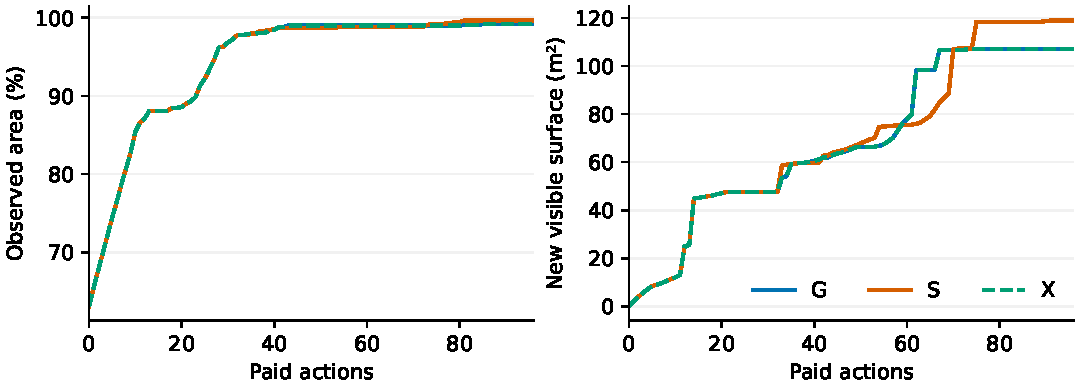
\includegraphics[width=.90\linewidth]{Q1_curves.pdf}
\caption{One prospectively fixed Q1 synthetic parent with native G/S/X. Left: observed reachable-cell coverage. Right: reference-visible surface added since the initial frame. G and X coincide exactly; S has a temporary surface deficit before the final gain. Each arm returns after 96 paid actions with no simulated collision. These related trajectories provide no between-scene uncertainty estimate.}\label{fig:Q1}
\end{figure}

\end{document}
